% !TeX encoding = UTF-8
% !TeX spellcheck = pl_PL

\def\filename{rozdzial3}
\chapter{Propozycja systemu do diagnostyki zmian skórnych}

\section{Dostępne zbiory danych zmian skórnych}

\subsection{ISIC}
Do rozwoju metod sztucznej inteligencji w dermatologii w istotny sposób przyczyniła się organizacja International Skin Imaging Collaboration (ISIC), której celem jest zwiększenie skuteczności wczesnego wykrywania czerniaka i tym samym zmniejszenie śmiertelności związanej z nowotworami skóry.
Od 2016 roku ISIC udostępnia obszerne zbiory obrazów z badań dermoskopowych wraz z danymi klinicznymi i wynikami diagnoz, organizując coroczne konkursy mające na celu doskonalenie algorytmów wizji komputerowej.
Archiwa ISIC z lat 2016-2024 odegrały kluczową rolę w rozwoju badań nad wykorzystaniem sztucznej inteligencji w diagnostyce nowotworów skóry, a opracowane przez organizację standardy są powszechnie akceptowane w dziedzinie CADx.
Zbiory z konkursów ISIC obejmują głównie obrazy dermoskopowe czerniaków i znamion melanocytowych, jednak w internetowych archiwach dostępne są również fotografie wielu innych rodzajów zmian skórnych \cite{Li_Koban_Schenck_Giunta_Li_Sun_2022}.

\subsection{HAM10000}
HAM10000 stanowi jeden z najczęściej wykorzystywanych oficjalnych zbiorów International Skin Imaging Collaboration \cite{Li_Koban_Schenck_Giunta_Li_Sun_2022}.
Został opracowany w celu zgromadzenia reprezentatywnej kolekcji najważniejszych kategorii diagnostycznych zmian barwnikowych, ponieważ wcześniejsze zasoby, takie jak archiwa ISIC czy zbiór PH2, były znacznie mniejsze i koncentrowały się głównie na diagnozie czerniaka złośliwego.
HAM10000 obejmuje 10.015 obrazów dermoskopowych, z czego diagnoza ponad połowy została potwierdzona badaniem histopatologicznym.
Zbiór uwzględnia również dane kliniczne pacjentów takie jak wiek, płeć oraz lokalizacja zmiany.
Obrazy zbierano na przestrzeni 20 lat w dwóch ośrodkach - w klinice dermatologicznej Uniwersytetu Medycznego w Wiedniu oraz w gabinecie dermatologicznym Cliffa Rosendahla w Queensland.
Austriacka część zbioru obejmuje zmiany u pacjentów często charakteryzujących się dużą liczbą znamion lub z znamionami podejrzanymi w kierunku czerniaka.
Z kolei australijski zestaw danych pochodzi od pacjentów zamieszkujących region o wysokiej zapadalności na nowotwory skóry, u których często obserwuje się przewlekłe uszkodzenia skóry spowodowane intensywną ekspozycją na promieniowanie słoneczne, takie jak plamy soczewicowate.

Wyróżniono następujące klasy w zbiorze:
\begin{itemize}
	\item akiec (actinic keratosis),
	\item bcc (basal cell carcinoma),
	\item bkl (benign keratosis),
	\item df (dermatofibroma),
	\item nv (melanocytic nevi),
	\item mel (melanoma),
	\item vasc (vascular lesion).
\end{itemize}

Klasa "`akiec'' obejmuje rogowacenie słoneczne, raka śródnabłonkowego oraz chorobę Bowena, czyli nieinwazyjne nowotwory, które można leczyć miejscowo bez konieczności wykonywania zabiegów chirurgicznych.
Pomimo nieinwazyjności tych nowotworów należy wziąć pod uwagę, że te zmiany mogą przekształcić się w inwazyjnego raka płaskonabłonkowego (ang. \textit{squamous cell carcinoma}), nieuwzględnionego w zbiorze.
"`Bcc'' dotyczy raka podstawnokomórkowego, czyli powszechną odmianę raka nabłonkowego skóry, który jest wysoko uleczalny, lecz w przypadku braku leczenia rozwija się destrukcyjnie.
Kategoria "`bkl'' stanowi ogólną klasę obejmującą łagodne rogowacenia skóry, takie jak rogowacenie łojotokowe (ang. \textit{seborrheic keratoses}) i plamki słoneczne oraz rogowacenie podobne do liszaju płaskiego.
Zdecydowano się na zgrupowanie tych zmian razem ze względu na podobieństwo pod względem biologicznym.
"`Df'' obejmuje dermatofibromę, czyli włókniaka twardego.
Jest ona łagodną zmianą skórną, najczęściej powstająca w wyniku reakcji zapalnej na uraz.
Klasa nv to znamiona melanocytowe, powszechnie znane jako pieprzyki.
Kategoria "`mel'' dotyczy czerniaka złośliwego wywodzącego się ze znamion melanocytowych.
Znamiona mogą być zwiększać ryzyko rozprzestrzeniania się w organizmie poprzez przenikanie poniżej naskórka do skóry właściwej, co w dermatologii jest określane inwazyjnością.
W zbiorze uwzględniono wszystkie odmiany czerniaka, ale wykluczono czerniaka bezbarwnikowego, podpaznokciowego, ocznego oraz błony śluzowej.
"`Vasc'' dotyczy łagodnych znamion naczyniowych, takich jak naczyniaki wiśniowe, ziarniniaki ropne oraz siniaki, które charakteryzują się czerwonym lub fioletowym kolorem.
\cite{Kittler_2018}.

\subsection{BCN20000}
BCN20000 to oficjalny zbiór ISIC udostępniony w 2024 roku.
Autorzy zebrali 18.946 obrazów dermoskopowych z kliniki w Barcelonie wykonanych w latach 2010-2016.
Zbiór obejmuje osiem kluczowych kategorii diagnostycznych w dermatologii, skupiając się szczególnie na zmianach w trudnych do zdiagnozowania miejscach, takich jak paznokcie i błony śluzowe, które często są pomijane przez pozostałe zbiory.
W BCN20000 uwzględniono również płeć i wiek pacjenta oraz położenie zmiany.
Wyróżniono następujące klasy w zbiorze:
\begin{itemize}
	\item ak (actinic keratosis),
	\item bcc (basal cell carcinoma),
	\item bkl (benign keratosis),
	\item df (dermatofibroma),
	\item scc (squamous cell carcinoma),
	\item nv (nevus),
	\item mel (melanoma),
	\item vasc (vascular lesion).
\end{itemize}

W porównaniu z zbiorem HAM10000, BCN20000 obejmuje więcej obrazów oraz dodatkowo uwzględnia raka kolczystokomórkowego (scc) \cite{Hernández2024}.

\subsection{DERM7PT}
DERM7PT stanowi zbiór danych służący do oceny skuteczności diagnostyki komputerowej na podstawie siedmiopunktowej skali oceny zmian skórnych.
Zbiór obejmuje 1.011 obrazów dermoskopowych, sklasyfikowanych w pięciu kategoriach oraz dwudziestu szczegółowych diagnozach:
\begin{itemize}
	\item bcc - basal cell carcinoma,
	\item nev - blue nevus, clark nevus, combined nevus, congenital nevus, dermal nevus, recurrent nevus, reed or spitz nevus,
	\item mel - melanoma, melanoma in situ, melanoma < 0,76 mm, melanoma 0,76 to 1,5 mm, melanoma > 1,5 mm,
	\item misc - dermatofibroma, lentigo, melanosis, miscellaneous, vascular lesion,
	\item sk - seborrheic keratosis.
\end{itemize}

W obrębie klasy "`nev'' wyszczególniono liczne typy powszechnych zmian melanocytowych, takich jak znamię błękitne, Clarka, złożone, wrodzone, śródskórne, nawrotowe, Reeda oraz Spitza.
Klasa "`mel'' obejmuje różne warianty czerniaka, w tym czerniaka in situ (nieinwazyjnego) i trzy podgrupy wydzielone na podstawie średnicy zmiany.
Kategoria "`misc'' zawiera łagodne zmiany skórne, takie jak włókniak twardy, plamki słoneczne czy melanoza.
Dodatkowo wyodrębniono osobne klasy dla rogowacenia łojotokowego (sk) oraz raka podstawnokomórkowego (bcc).
Autorzy zbioru przypisali każdej zmianie cechy odpowiadające siedmiopunktowej skali, umożliwiając analizę zarówno klasyfikacyjną, jak i cechową \cite{Hamarneh_2019}.

\subsection{PAD-UFES-20}
PAD-UFES-20 jest zbiorem obejmującym 2.298 przypadków zmian skórnych wykonanych kamerą smartfonu, co czyni go szczególnie istotnym w kontekście projektowania mobilnych systemów wspomagania diagnostyki dermatologicznej.
58\% znamion z zbioru zostało poddanych biopsji.
PAD-UFES-20 zawiera sześć kategorii zmian skórnych:
\begin{itemize}
	\item bcc (basal cell carcinoma),
	\item scc (squamous cell carcinoma),
	\item ack (actinic keratosis),
	\item sek (seborrheic keratosis),
	\item mel (melanoma),
	\item nev (nevus).
\end{itemize}
W ramach klasy "`scc'', czyli raka kolczystokomórkowego uwzględniono również chorobę Bowena, który jest nieinwazyjną postacią tego nowotworu.
Zbiór obejmuje również szeroki zakres danych klinicznych pacjentów, takich jak informacje o paleniu, obecności bólu lub krwawienia zmiany, a także dane socjoekonomiczne, takie jak dostęp do bieżącej wody i kanalizacji.
PAD-UFES-20 jest jedynym publicznie dostępnym zbiorem obrazów zmian skórnych wykonanych kamerą telefonu komórkowego, co wyraźnie odróżnia go od pozostałych zasobów wykorzystywanych w badaniach nad automatyczną analizą dermatoskopową \cite{Castro_2020}.

\subsection{MED-NODE}
MED-NODE to zbiór danych obejmujący 170 obrazów klinicznych przedstawiających zmiany melanocytowe, spośród których 70 przypadków stanowi czerniak złośliwych a 100 to łagodne zmiany melanocytowe, powszechnie nazywane pieprzykami.
Zdjęcia zostały pozyskane w klinice dermatologii Uniwersytetu Medycznego w Groningen, przy użyciu aparatu cyfrowego \cite{giotis2015med}.

\subsection{PH2}
PH2 jest zbiorem opublikowany w 2013 roku, obejmujący 200 obrazów dermoskopowych. 
40 przypadków to potwierdzony histopatologicznie czerniak, pozostałe zdjęcia stanowią łagodne znamiona melanocytowe.
W zbiorze zawarto również szczegółowe informacje kliniczne i dermoskopowe, w tym ocenę cech strukturalnych, diagnozę kliniczną i histologiczną.
Ze względu na swoją kompletność i dostępność PH2 stanowił podstawowy zestaw referencyjny w badaniach nad algorytmami klasyfikacji zmian skórnych, zanim został zastąpiony przez bardziej obszerne zbiory, takie jak HAM10000 \cite{Rozeira_2013}.

\subsection{Fitzpatrick17k}
Fitzpatrick17k składa się z 16.577 obrazów klinicznych pochodzących z dwóch internetowych atlasów dermatologicznych - DermaAmin oraz Atlas Dermatologico.
Każde zdjęcie oznaczono etykietami typu skóry według skali Fitzpatricka, klasyfikującej reaktywność skóry na promieniowanie słoneczne.
W zbiorze uwzględniono 114 schorzeń skóry, przy czym liczba obrazów przypadających na jedną jednostkę chorobową wynosi od 53 do 653 przypadków.
Główne kategorie schorzeń obecne w zbiorze to:
\begin{itemize}
	\item inflammatory,
	\item malignant epidermal,
	\item genodermatoses,
	\item benign dermal,
	\item benign epidermal,
	\item malignant melanoma,
	\item benign melanocyte,
	\item malignant cutaneous lymphoma,
	\item malignant dermal.
\end{itemize}
Do kategorii chorób zapalnych należą takie jednostki chorobowe jak łuszczyca i trądzik.
Klasa "`malignant epidermal'' zawiera złośliwe nowotwory naskórka, na przykład raka podstawnokomórkowego i rogowacenie słoneczne.
Grupa genodermatoz uwzględnia choroby dziedziczne skóry, takie jak neurofibromatoza i zespół Ehlersa-Danlosa.
W klasie "`benign dermal'' i "`benign epidermal'' zawarto łagodne zmiany skórne na poziomie naskórka i skóry właściwej, na przykład włokniaka twardego lub ziarniniaka naczyniowego.
Kategoria łagodnych znamion melanocytowych uwzględnia różne rodzaje pieprzyków.
Kategoria "`malignant dermal'' obejmuje mięsaka Kaposiego, czyli nowtwór złośliwy wywołany przez wirusa HHV-8.
Autorzy uwzględnili także osobą grupę dla czerniaka złośliwego, która zawiera przypadki nowotworu w różnych stadium choroby oraz dla ziarniniaka grzybiastego, czyli najpowszechniejszego chłoniaka skóry \cite{groh2021evaluating, Schneider_Dittmer_2017, Bowman_Hogan_Sanusi_2001}.

Zbiór Fitzpatrick17k odpowiada na istotną lukę w dziedzinie diagnostyki komputerowej, dotyczącą niedostatecznej reprezentacji zróżnicowanych fototypów skóry w dostępnych danych.
Co więcej, zbiór rozszerza badane jednostki z znamion do ogólnych dermatologicznych schorzeń, takich jak choroby autoimmunologiczne lub urazy.
Jednocześnie zbiór jest ograniczony przez brak jednolitej obróbki obrazów, ponieważ zdjęcia są wykonane w różnych warunkach, co skutkuje zmiennością jakości, co nie jest odpowiednimi warunkami do trenowania modeli uczenia maszynowego.
Dodatkowy problem stanowi brak publicznie dostępnego archiwum obrazów.
Udostępniono jedynie odnośniki do atlasów internetowych, co powoduje ryzyko utraty danych w przypadku usunięcia materiałów źródłowych \cite{groh2021evaluating}.

\subsection{Dermofit}
Dermofit to niepubliczny zbiór opracowany przez Uniwersytet Edynburski, obejmujący 1300 obrazów klinicznych sklasyfikowanych w dziesięciu kategoriach zmian skórnych.
Diagnozy zostały potwierdzone przez dermatologów i dermopatologów.
Do każdego obrazu załączono również maskę segmentacyjną, wyznaczającą obszar zmiany.
Dermofit obejmuje następujące klasy:
\begin{itemize}
	\item actinic keratosis,
	\item basal cell carcinoma,
	\item squamous cell carcinoma,
	\item seborrheic keratosis,
	\item malignant melanoma,
	\item nevus,
	\item intraepithelial carcinoma,
	\item pyogenic granuloma,
	\item haemangioma,
	\item dermatofibroma.
\end{itemize}
Na tle innych zbiorów danych Dermofit wyróżnia się obecnością rzadziej spotykanych kategorii zmian skórnych, takich jak rak śródnabłonkowy, ziarniniak naczyniowy oraz naczyniak krwionośny, co zwiększa jego wartość w badaniach nad klasyfikacją wieloklasową \cite{Dermofit, inbook}

\begin{sidewaystable}
	\tiny
	\caption{Zestawienie zbiorów zmian skórnych}
	\centering
	\begin{tabular}{|c|c|c|c|p{2cm}|c|c|c|p{3cm}|}
		\hline
		\textbf{Nazwa zbioru} &
		\textbf{Autorzy} &
		\textbf{Rok publikacji} &
		\textbf{Dostępność} &
		\textbf{Metoda zbierania zdjęć} &
		\textbf{Liczba obrazów} &
		\textbf{Liczba klas} &
		\textbf{\% potwierdzony histopatologicznie} &
		\textbf{Klasy} \\ \hline
		
		HAM10000 & \cite{Kittler_2018} & 2018 & Dostępny publicznie & Badanie dermoskopowe & 10\.015 & 7 & 53,3\% &
		327 - actinic keratosis
		
		514 - basal cell carcinoma
		
		1.099 - benign keratosis
		
		115 - dermatofibroma
		
		1.113 - melanoma
		
		6705 - nevus
		
		142 - vascular lesion \\ \hline
		
		BCN20000 & \cite{Hernández2024} & 2024 & Dostępny publicznie & Zdjęcia kliniczne, zdjęcia z przybliżeniem, badanie dermoskopowe & 18\.946 & 8 & 100\% &
		737 - actinic keratosis
		
		2.809 - basal cell carcinoma
		
		431 - squamous cell carcinoma
		
		1.138 - benign keratosis
		
		124 - dermatofibroma
		
		2.857 - melanoma
		
		4.206 - nevus
		
		111 - vascular lesion \\ \hline
		
		DERM7PT & \cite{Hamarneh_2019} & 2019 & Dostępny publicznie & Zdjęcia kliniczne, badanie dermoskopowe & 1\.011 & 20 & Brak informacji &
		42 - basal cell carcinoma
		
		
		1 - melanoma
		
		64 - melanoma in situ
		
		102 - melanoma < 0{,}76 mm
		
		53 - melanoma 0{,}76–1{,}5 mm
		
		28 - melanoma > 1{,}5 mm
		
		
		28 – blue/clark nevus
		
		13 – combined nevus
		
		17 - congenital nevus
		
		33 – dermal nevus
		
		6 – recurrent nevus
		
		79 – reed/spitz nevus
		
		
		20 – dermatofibroma
		
		24 – lentigo
		
		16 – melanosis
		
		8 – miscellaneous
		
		29 – vascular lesion
		
		
		45 – seborrheic keratosis \\ \hline
		
		PAD-UFES-20 & \cite{Castro_2020} & 2020 & Dostępny publicznie & Zdjęcia kliniczne wykonane smartfonem & 2\.298 & 6 & 58,4\% &
		730 – actinic keratosis
		
		845 – basal cell carcinoma
		
		192 – squamous cell carcinoma
		
		52 – melanoma
		
		244 – nevus
		
		235 – seborrheic keratosis \\ \hline
		
		MED-NODE & \cite{giotis2015med} & 2015 & Dostępny publicznie & Zdjęcia wykonane aparatem cyfrowym & 170 & 2 & Brak informacji &
		70 – melanoma
		
		100 – nevus \\ \hline
		
		PH2 & \cite{Rozeira_2013} & 2013 & Dostępny publicznie & Badanie dermoskopowe & 200 & 2 & 20,5\% &
		40 – melanoma
		
		160 – nevus \\ \hline
		
		Fitzpatrick17k & \cite{groh2021evaluating} & 2021 & Dostępny publicznie & Zdjęcia wykonane w różnych warunkach, z różnych źródeł & 16\.577 & 114 & Brak informacji &
		10\.886 – inflammatory
		
		1.352 – malignant epidermal
		
		1.194 – genodermatoses
		
		1.067 – benign dermal
		
		931 – benign epidermal
		
		573 – malignant melanoma
		
		236 – benign melanocyte
		
		182 – malignant cutaneous lymphoma
		
		156 – malignant dermal \\ \hline
		
		Dermofit & \cite{Dermofit, inbook} & 2013 & Wymaga umowy i opłaty & Zdjęcia wykonane aparatem cyfrowym & 1\.300 & 10 & Brak informacji &
		45 – actinic keratosis
		
		239 – basal cell carcinoma
		
		88 – squamous cell carcinoma
		
		78 – intraepithelial carcinoma
		
		65 – dermatofibroma
		
		76 – melanoma
		
		331 – nevus
		
		24 – pyogenic granuloma
		
		96 – haemangioma
		
		257 – seborrheic keratosis \\ \hline

	\end{tabular}
	\source{opracowanie własne}
\end{sidewaystable}


\section{Dobór zbiorów i opis wybranych zmian skórnych}
Dostępne zbiory danych obejmują szerokie spektrum jednostek chorobowych, wobec czego opracowanie mobilnego systemu umożliwiającego identyfikację różnych zmian skórnych wymaga starannego doboru źródeł danych oraz ujednolicenia klas przed rozpoczęciem dalszej analizy.
Ograniczenie liczby rozpoznawanych typów zmian jest konieczne, ponieważ nadmierna liczba klas zwiększałaby złożoność obliczeniową modelu oraz mogłaby prowadzić do niewystarczającej liczby przykładów dla poszczególnych kategorii.
Z kolei zbyt mała liczba klas obniżyłaby użyteczność systemu.

W eksperymentach wykorzystano zbiory HAM10000, BCN20000, DERM7PT, ISIC 2020 oraz PAD-UFES-20.
Wstępne próby łączenia zdjęć dermoskopowych ze zdjęciami wykonanymi aparatem telefonu wykazały, że tak duża heterogeniczność danych znacząco obniżała jakość modelu i utrudniała efektywne uczenie się charakterystyk obrazów.
W konsekwencji zdecydowano się na wytrenowanie dwóch odrębnych modeli - jednego opartego wyłącznie na obrazach dermoskopowych oraz drugiego trenowanego jedynie na zdjęciach wykonanych aparatem smartfonu.

Model wytrenowany na obrazach dermoskopowych osiągał bardzo wysokie wyniki na danych testowych pochodzących z tego samego typu obrazów, jednak jego skuteczność drastycznie spadała w przypadku zdjęć wykonanych telefonem.
Wynika to z faktu, że fotografie mobilne charakteryzują się znacznie większą zmiennością pod względem oświetlenia, jakości oraz sposobu kadrowania.
W kolejnym etapie wytrenowano modele wyłącznie na zbiorze PAD-UFES-20.
Uzyskane wyniki wskazały, że modele oparte na tym zbiorze radzą sobie najlepiej w warunkach odpowiadających rzeczywistemu zastosowaniu aplikacji mobilnej.
Z tego powodu zdecydowano się wykorzystać wyłącznie PAD-UFES-20 jako podstawę dalszych badań.

Analiza zmian skórnych przez system opiera się wyłącznie na obrazie, więc wykorzystano jedynie metadane w postaci odnośników do zdjęć oraz odpowiadających im diagnoz.
W zbiorze PAD-UFES-20 wyróżniono sześć kategorii zmian skórnych:
\begin{itemize}
	\item BCC (basal cell carcinoma) - 845 obrazów raka podstawnokomórkowego,
	\item ACK (actinic keratosis) - 730 obrazów rogowacenia słonecznego,
	\item NEV (nevus) - 244 obrazy znamion melanocytowych, czyli pieprzyków,
	\item SEK (seborrheic keratosis) - 235 obrazów rogowacenia łojotokowego,
	\item SCC (squamous cell carcinoma) - 192 obrazy raka kolczystkomórkowego,
	\item MEL (melanoma) - 52 obrazy czerniaka.
\end{itemize}

\subsection{Rak podstawnokomórkowy - basal cell carcinoma}

\begin{figure}[h!]
	\centering
	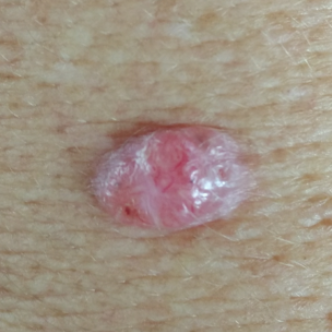
\includegraphics[width=0.2\linewidth]{bcc_sample}
	\caption{Klasa "`basal cell carcinoma''}
	\source{PAD-UFES-20 \cite{Castro_2020}}
	\label{fig:bcc_sample}
\end{figure}

Rak podstawnokomórkowy (basal cell carcinoma, BCC), przedstawiony na Rysunku \ref{fig:bcc_sample} jest najczęściej występującym złośliwym nowotworem skóry, szczególnie u osób o jasnej karnacji.
Rozwija się w wyniku przewlekłej ekspozycji na promieniowanie ultrafioletowe oraz częściej dotyczy osób w starszym wieku.
Zmiana zwykle wykazuje obecność pajączków naczyniowych na swojej powierzchni, a wraz z upływem czasu stopniowo się powiększa, prowadząc do powstania nieregularnej, szorstkiej struktury.

BCC wywodzi się z keratynocytów warstwy podstawnej naskórka, rozwijających się w obrębie skóry uszkodzonej przez działanie promieniowania słonecznego.
Charakteryzuje się powolnym wzrostem oraz niskim ryzykiem przerzutów, co sprawia, że rokowanie jest zazwyczaj dobre, zwłaszcza przy wczesnym wykryciu. 
Standardową metodą leczenia jest chirurgiczne usunięcie zmiany, które w większości przypadków prowadzi do całkowitego wyleczenia \cite{Bourke_2010}.

\subsection{Rogowacenie słoneczne - actinic keratosis}

\begin{figure}[h!]
	\centering
	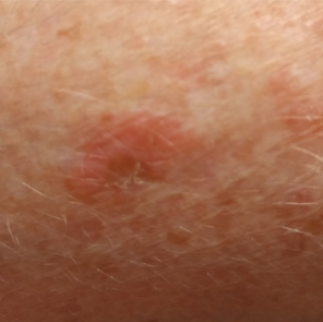
\includegraphics[width=0.2\linewidth]{ack_sample}
	\caption{Klasa "`actinic keratosis''}
	\source{PAD-UFES-20 \cite{Castro_2020}}
	\label{fig:ack_sample}
\end{figure}

Klasa rogowacenia słonecznego obejmuje nieinwazyjne zmiany przednowotworowe powstające w wyniku przewlekłej ekspozycji na promieniowanie ultrafioletowe.
Zmiana może przekształcić się w złośliwego raka kolczystokomórkowego, przez co wymaga obserwacji.
Pojedyncze obszary rogowacenia słonecznego różnią się od siebie i pojawiają się w każdym miejscu przewlekle eksponowanym na słońce, np. na twarzy, uszach i szyi.
Przykładową fotografię rogowacenia słonecznego przedstawiono na Rysunku \ref{fig:ack_sample}.
Rozpoznanie wymaga potwierdzenia histopatologicznego, natomiast leczenie może obejmować krioterapię, wyłyżeczkowanie lub chirurgiczne usunięcie zmiany \cite{Bourke_2010}.

\subsection{Zmiana melanocytowa - nevus}
\begin{figure}[h!]
	\centering
	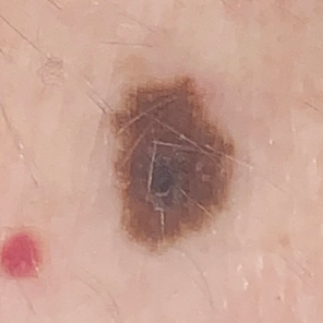
\includegraphics[width=0.2\linewidth]{nev_sample}
	\caption{Klasa "`nevus''}
	\source{PAD-UFES-20 \cite{Castro_2020}}
	\label{fig:nev_sample}
\end{figure}

Klasa nevus dotyczy łagodnych znamion melanocytowych, powszechnie określanych jako pieprzyki.
Zmiany melanocytowe nie stanowią zagrożenia zdrowotnego, usuwa się je głównie ze względów estetycznych bądź w przypadku podejrzenia zezłośliwienia \cite{Bourke_2010}.
Pod względem dermoskopowym mogą znacznie się różnić między sobą, m.in. w zakresie barwy, jednak w przeciwieństwie do czerniaka cechują się symetrią oraz jednorodnością struktury.
Przykładowy obraz z klasy NEV przedstawiono na Rysunku \ref{fig:nev_sample}.

\subsection{Rogowacenie łojotokowe - seborrheic keratosis}
\begin{figure}[h!]
	\centering
	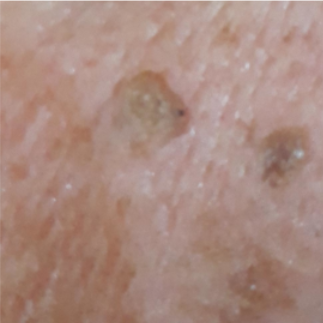
\includegraphics[width=0.2\linewidth]{sek_examples}
	\caption{Klasa "`seborrheic keratosis''}
	\source{PAD-UFES-20 \cite{Castro_2020}}
	\label{fig:sek_sample}
\end{figure}

Rogowacenie łojotokowe, określane również jako brodawka starcza, to łagodna zmiana nowotworowa wywodząca się z komórek naskórka.
Zmiany te są zazwyczaj wyniosłe powierzchnię skóry i mają ostro odgraniczone granice.
Wraz z upływem czasu mogą stopniowo powiększać się i ciemnieć.
Rogowacenie łojotokowe nie stanowi zagrożenia zdrowotnego i nie ulega zezłośliwieniu, dlatego leczenie nie jest konieczne \cite{Hafner_Vogt_2008}.
Przykładową zmianę należącą do klasy SEK przedstawiono na Rysunku \ref{fig:sek_sample}.

\subsection{Rak kolczystokomórkowy - squamous cell carcinoma}
\begin{figure}[h!]
	\centering
	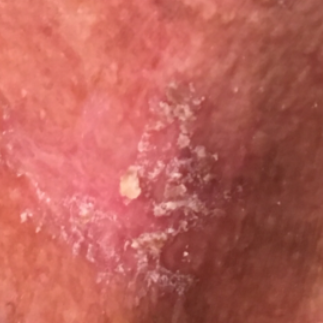
\includegraphics[width=0.2\linewidth]{scc_examples}
	\caption{Klasa "`squamous cell carcinoma''}
	\source{PAD-UFES-20 \cite{Castro_2020}}
	\label{fig:scc_examples}
\end{figure}

Rak kolczystokomórkowy to złośliwy nowotwór skóry rozwijający się najczęściej u osób starszych, szczególnie w miejscach przewlekle narażonych na działanie czynników karcynogennych, takich jak promieniowanie ultrafioletowe czy związki pochodne dziegciu.
Nowotwór ten wywodzi się z keratynocytów warstwy kolczystej naskórka i może klinicznie przypominać rogowacenie słoneczne lub przyjmować postać większych mas bądź owrzodzeń.
SCC charakteryzuje się stosunkowo niskim ryzykiem przerzutów, 
Leczenie opiera się na chirurgicznym wycięciu zmiany, a w wybranych przypadkach stosuje się również radioterapię \cite{Bourke_2010}.
Przykład raka kolczystokomórkowego pokazano na Rysunku \ref{fig:scc_examples}.

\subsection{Czerniak - melanoma}
\begin{figure}[h!]
	\centering
	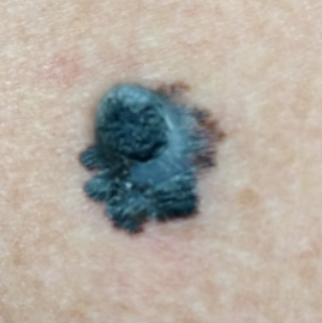
\includegraphics[width=0.2\linewidth]{mel_sample}
	\caption{Klasa "`melanoma''}
	\source{PAD-UFES-20 \cite{Castro_2020}}
	\label{fig:mel_sample}
\end{figure}

Czerniak złośliwy to agresywny nowotwór wywodzący się z znamion melanocytowych, mogący występować zarówno w postaci inwazyjnej i nieinwazyjnej (in situ).
Zmianę przedstawiono na Rysunku \ref{fig:mel_sample}.
Wczesne wykrycie czerniaka umożliwia skuteczne leczenie chirurgiczne.
Czerniak różni się od łagodnych znamion melanocytowych nieregularną strukturą, asymetrią oraz niejednorodnością barwy \cite{Bourke_2010}.

\begin{figure}[h!]
	\centering
	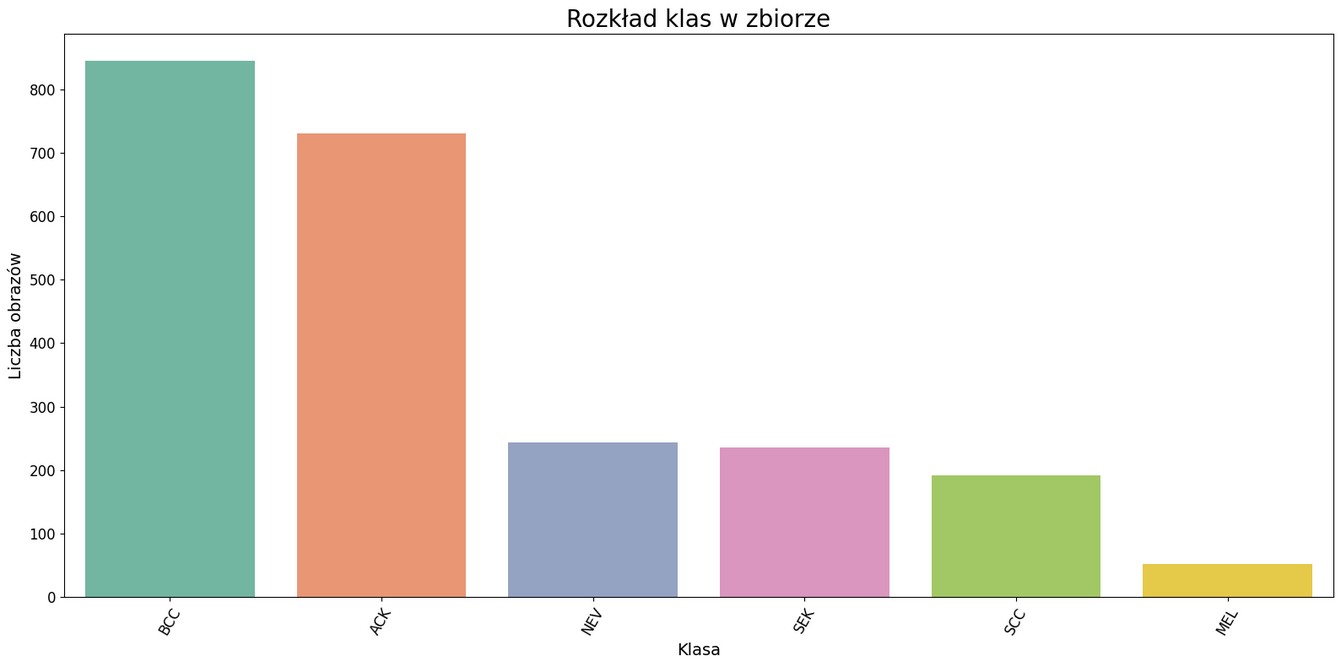
\includegraphics[width=0.9\linewidth]{classes_bar}
	\caption{Rozkład klas w zbiorze po ich ujednoliceniu}
	\source{opracowanie własne}
	\label{fig:classes_bar}
\end{figure}

\begin{figure}[h!]
	\centering
	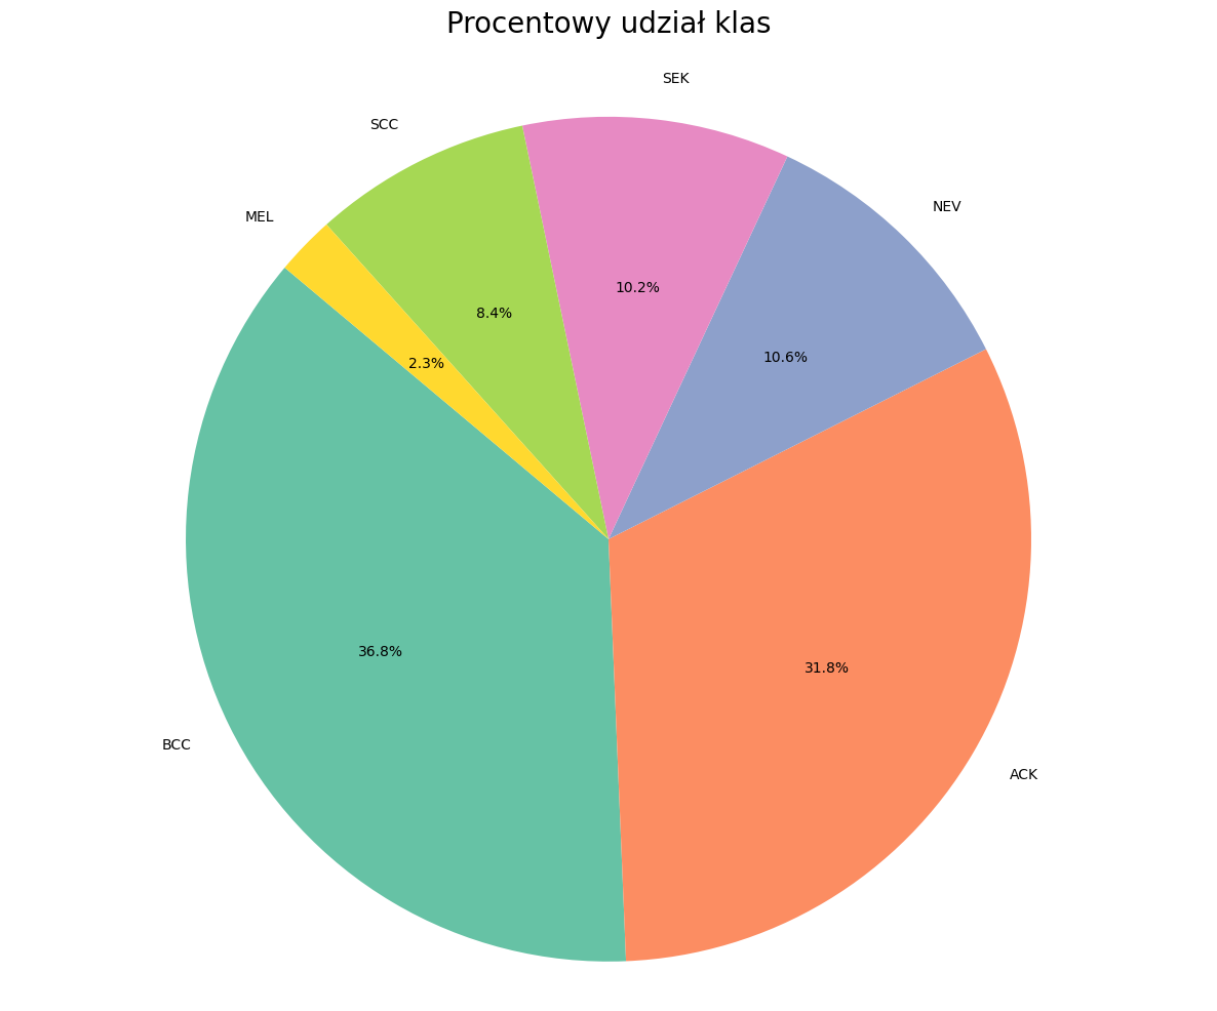
\includegraphics[width=0.7\linewidth]{classes_pie}
	\caption{Procentowy udział klas w zbiorze przed ich ujednoliceniem}
	\source{opracowanie własne}
	\label{fig:classes_pie}
\end{figure}

Łącznie badany zbiór obejmował 2.298 obrazów, co przedstawiono na wykresie słupkowym (Rys. \ref{fig:classes_bar}) oraz wykresie kołowym (Rys. \ref{fig:classes_pie}).
W kolejnych etapach przeprowadzono dalsze czyszczenie oraz przygotowanie danych pod kątem wymagań modelu, co szczegółowo opisano w Rozdziale 4, w podrozdziale "`Obróbka danych''.

\section{Infrastruktura}
Pierwszym etapem opracowania systemu identyfikacji zmian skórnych jest przygotowanie i wytrenowanie odpowiedniego modelu uczenia maszynowego.
W ramach niniejszej pracy zastosowano technikę \textit{transfer learning}, polegającą na wykorzystaniu wcześniej wytrenowanych modeli konwolucyjnych i dostosowaniu ich do specyfiki nowych danych.
Po zakończeniu procesu uczenia model został skonwertowany do formatu TensorFlow Lite, umożliwiającego uruchamianie bezpośrednio na urządzeniach mobilnych z systemem Android, co oznacza, że inferencja odbywa się lokalnie, bez konieczności przesyłania danych do zewnętrznej infrastruktury obliczeniowej.
Aplikacja mobilna została opracowana w języku Kotlin z wykorzystaniem biblioteki Jetpack Compose, która umożliwia stworzenie interfejsu użytkownika.
Model w formacie TFlite jest integralną częścią aplikacji.
Znajduje się on w zasobach programu i jest wykorzystywany bezpośrednio do procesu wnioskowania za pomocą biblioteki TensorFlow Lite, zapewniającej obsługę modeli uczenia maszynowego na urządzeniach mobilnych.

\begin{figure}[h!]
	\centering
	\includegraphics[width=0.9\linewidth]{diagram_systemu}
	\caption{Uproszczony diagram systemu przedstawiający działanie aplikacji}
	\source{opracowanie własne}
	\label{fig:diagram_systemu}
\end{figure}

Diagram na Rys. \ref{fig:diagram_systemu} przedstawia uproszczoną architekturę systemu oraz ścieżkę interakcji użytkownika z aplikacją.
W pierwszym kroku użytkownik wykonuje zdjęcie zmiany skórnej za pomocą aparatu telefonu komórkowego lub wczytuje je z pamięci urządzenia.

\begin{figure}[h!]
	\centering
	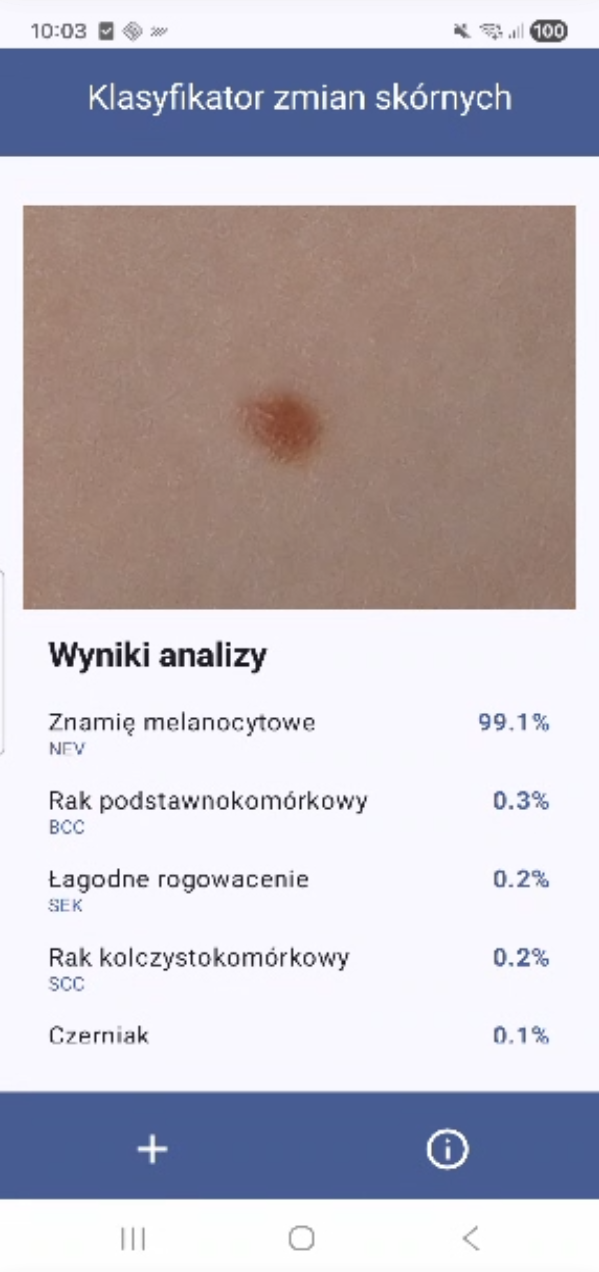
\includegraphics[width=0.3\linewidth]{screen5}
	\caption{Interfejs użytkownika aplikacji}
	\source{opracowanie własne}
	\label{fig:screen5}
\end{figure}

Następnie obraz jest przekazany do lokalnie przechowywanego modelu TFLite, który dokonuje inferencji i zwraca wynik klasyfikacji, który jest wyświetlony na interfejsie użytkownika w postaci procentowych prawdopodobieństw przynależności badanej zmiany do każdej z klas, co przedstawiono na Rys. \ref{fig:screen5}.

\section{Podsumowanie}
Prezentowany system stanowi przykład praktycznego wykorzystania głębokich sieci neuronowych do wstępnego rozpoznawania zmian skórnych, uwzględniający zarówno obecne regulacje prawne, jak i ograniczenia technologii sztucznej inteligencji oraz związane z nią zagadnienia etyczne.
Aplikacja wykorzystuje powszechną dostępność smartfonów oraz rosnącą jakość ich aparatów fotograficznych, aby zwiększać świadomość pacjentów w zakresie monitorowania zmian skórnych i wspierać wczesną identyfikację niepokojących objawów.
Choć współczesne modele uczenia maszynowego nie osiągnęły jeszcze poziomu dojrzałości umożliwiającego ich pełnoprawne zastosowanie kliniczne, rozwijanie prototypowych rozwiązań tego typu pozostaje kluczowe dla dalszego postępu AI.
Systemy wykorzystujące sieci neuronowe mogą w przyszłości asystować lekarzom w procesie diagnostycznym, odciążać służbę zdrowia oraz zwiększać świadomość pacjentów w zakresie wczesnego wykrywania zmian skórnych.
Należy podkreślić, że wynik wygenerowany przez model nie stanowi diagnozy medycznej, lecz jedynie statystyczne przybliżenie oparte na ograniczonym zbiorze danych treningowych.
W kontekście wyzwań opisanych w Rozdziale 2, obejmujących m.in. stronniczość danych, brak wyjaśnialności wyniku oraz kwestie regulacyjne, które dopiero rozwijają się w dziedzinie sztucznej inteligencji, kliniczne zastosowanie przedstawionego rozwiązania pozostaje znacząco ograniczone.

Wykorzystanie lokalnie działającego modelu, bez konieczności przesyłania zdjęć do chmury, stanowi zaletę pod względem prywatności i bezpieczeństwa danych użytkownika.
Jednocześnie jednak takie podejście uniemożliwia dalsze doskonalenie modelu na podstawie rzeczywistych zdjęć wykonywanych przez użytkowników, co mogłoby przyczynić się do zwiększenia jego skuteczności i lepszej generalizacji.
Ponadto proponowane rozwiązanie nie eliminuje fundamentalnych ograniczeń technologii głębokiego uczenia, takich jak podatność na błędy wynikające z jakości zdjęcia, różnorodności urządzeń czy brak pełnej interpretowalności decyzji modelu.
Z tych względów opracowany system należy traktować jako narzędzie pomocnicze, którego główną rolą jest zwiększanie świadomości użytkownika oraz ułatwianie wczesnej identyfikacji zmian mogących wymagać konsultacji dermatologicznej.
Ostateczna decyzja diagnostyczna powinna zawsze należeć do lekarza, a system może jedynie uzupełniać proces podejmowania decyzji, nie zastępując profesjonalnej oceny klinicznej.